\documentclass[11pt,brazil]{beamer}
\usepackage{amssymb,amsfonts,amstext,amsthm}
\usepackage{amsmath,mathrsfs}
\usepackage[brazil]{babel}
\usepackage[utf8]{inputenc}
\usepackage{graphicx}
\usepackage{hyperref}
\usepackage{xcolor}
\usepackage{ragged2e}
\usepackage{booktabs}
\usepackage{tikz-cd}
\usetikzlibrary{cd}
\usepackage{tikz}
\usetikzlibrary{automata, positioning, arrows}
\tikzset
{
    ->, % makes the edges directed
    >=stealth',
    semithick,
    node distance=3cm, % specifies the minimum distance between two nodes. Change if necessary.
    every state/.style={thick, fill=gray!10}, % sets the properties for each ’state’ node
    initial text=$ $, % sets the text that appears on the start arrow
}

% Configuração visual do modelo fornecido pelo apresentador.
\apptocmd{\frame}{}{\justifying}{}
\usetheme{AnnArbor}
\usecolortheme{whale}
\setbeamertemplate{theorems}[numbered]
\setbeamercolor{frametitle}{use=structure,fg=white,bg=structure.fg!75!black}
\setbeamercolor{block title}{use=structure,fg=white,bg=structure.fg}
\setbeamercolor{block body}{use=structure,fg=black,bg=structure.fg!10}
\setbeamercolor{block title example}{use=structure,fg=white,bg=structure.fg}
\setbeamercolor{block body example}{use=structure,fg=black,bg=structure.fg!10}
\setbeamercovered{transparent}
\setbeamertemplate{page number in head/foot}{}

\newcommand{\R}{\mathbb{R}}
% O artigo não identifica cargo nem nome oficial do laboratório.
\newcommand{\grupo}{Equipe de pesquisa}
\newcommand{\vinculo}{Instituto de Ciências Matemáticas e de Computação (ICMC)\\Universidade de São Paulo (USP)}

\author{Junio Cesar Ferreira}
\title[Simpósio Brasileiro de Pesquisa Operacional]{\textbf{Planejamento Discreto de Redes de Sensores com Nós Móveis via Programação Inteira Mista e Avaliação por Simulação}}
\subtitle{}
\institute[ICMC-USP]{Simpósio Brasileiro de Pesquisa Operacional}
\date{Setembro de 2026}
\hypersetup{pdftitle={Planejamento Discreto de Redes de Sensores com Nós Móveis via Programação Inteira Mista e Avaliação por Simulação},pdfauthor={Junio Cesar Ferreira},pdflang={pt-BR}}

\AtBeginSection[]{
  \begin{frame}[plain]
    \vfill
    \centering
    \begin{beamercolorbox}[sep=8pt,center,shadow=true,rounded=true]{title}
      \usebeamerfont{title}\insertsectionhead\par
    \end{beamercolorbox}
    \vfill
    \note{Tempo: 5 segundos. Anuncie a seção e avance para o conteúdo.}
  \end{frame}
}

% make notes gera uma versão separada com as notas de fala.
\ifdefined\comnotas
  \setbeameroption{show notes}
\else
  \setbeameroption{hide notes}
\fi

\begin{document}

\begin{frame}[plain]
  \maketitle
  \note{Tempo: 25 segundos. Apresente o trabalho e a questão investigada: selecionar posições de nós fixos para atender dispositivos móveis, utilizando programação inteira mista e simulação.}
\end{frame}

\begin{frame}{Roteiro da apresentação}
  \begin{itemize}
    \item Apresentação e contexto da pesquisa
    \vfill
    \item Definição do problema
    \vfill
    \item Modelo MILP
    \vfill
    \item Metodologia experimental
    \vfill
    \item Resultados
    \vfill
    \item Considerações finais
  \end{itemize}
  \note{Tempo: 20 segundos. Apresente a sequência: contexto, definição do problema, formulação matemática, metodologia, resultados e conclusões.}
\end{frame}

\section{Apresentação e contexto da pesquisa}

\begin{frame}{Apresentação e contexto da pesquisa}
  \textbf{Junio Cesar Ferreira} (doutorando)
  \medskip

  \vinculo

  \begin{block}{\grupo}
    \begin{itemize}
      \item Júlio Cezar Estrella (orientador)
      \item Cláudio F. M. Toledo (coorientador)
      \item Alexandre C. B. Delbem (coorientador)
    \end{itemize}
  \end{block}
  \vfill
  O trabalho é motivado pelo desafio de projetar redes de sensores sem fio em cenários nos quais parte dos elementos da rede apresenta mobilidade.
\end{frame}

\section{Definição do problema}

\begin{frame}{Descrição do problema}
  Sensores em tratores, robôs e veículos de apoio precisam enviar seus dados a um ponto de coleta, denominado \textit{sink}.
  \begin{figure}
    \centering
    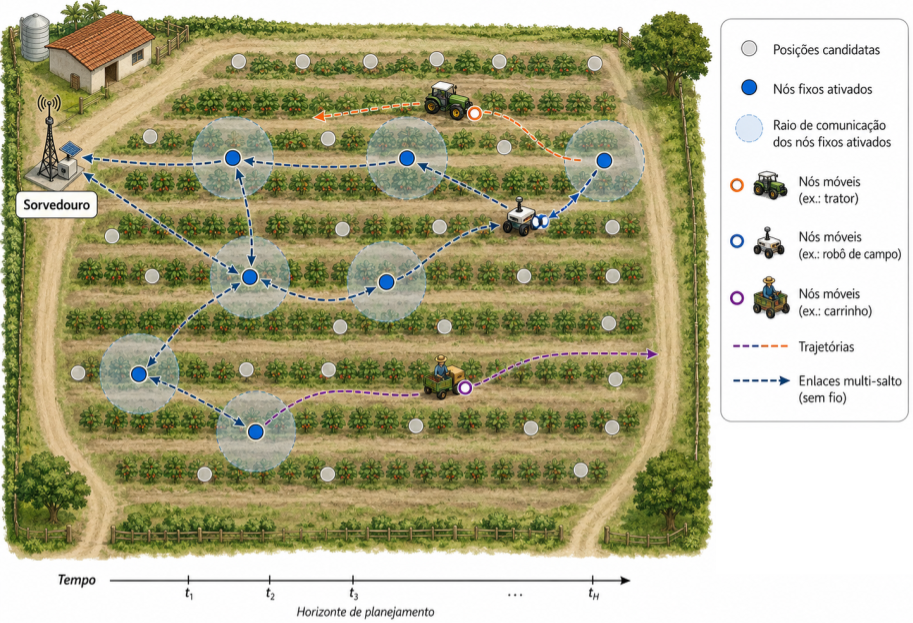
\includegraphics[height=4.3cm]{img/cenario-agricola.png}
  \end{figure}
  \textbf{Problema:} determinar posições para a instalação de nós fixos que garantam comunicação multi-hop ao longo das trajetórias dos nós móveis, otimizando simultaneamente métricas de desempenho da rede.
  \note{Tempo: 70 segundos. Na Figura 1 do artigo, identifique os móveis, as posições candidatas, os nós instalados e o sink. Explique que o alcance limitado exige retransmissão entre nós. As posições dos móveis mudam, mas a infraestrutura instalada permanece. A figura representa a motivação agrícola; o experimento realizado é geométrico e controlado, não uma implantação em campo.}
\end{frame}

\begin{frame}{Definição do problema}
  \begin{block}{Dados do problema}
    Considere uma região $\Omega\subset\R^2$, um ponto pré-fixado $\sigma\in\R^2$ indexado por $s$, posições candidatas $Q=\{q_j\;|\;j\in\mathcal J\}$ e dispositivos móveis $\{\gamma_m:[0,H]\rightarrow\Omega\;|\;m\in \mathcal M\}$ com trajetórias conhecidas.
  \end{block}
  O horizonte é discretizado em períodos $t\in\mathcal T$. Em cada período, temos o grafo $G_t=(V,E_t)$, com
  \[
    V=\{s\}\cup\mathcal J\cup\mathcal M,
  \]
  \[
    E_t=\big\{(i,j)\in V\times V:0<d_{ij}(t)\le R_{\mathrm{com}}\big\}.
  \]
  \begin{block}{Objetivo do planejamento}
    Selecionar um subconjunto $P\subseteq Q$ de nós fixos para que, em cada período, a demanda dos móveis chegue ao sink por caminhos com capacidade suficiente.
  \end{block}
  \note{Tempo: 80 segundos. Defina os conjuntos e a distância entre as posições dos nós. J e M são conjuntos de rótulos disjuntos. O raio de comunicação determina os arcos geometricamente viáveis. As instalações são compartilhadas por todos os períodos, enquanto enlaces e fluxos podem mudar. A garantia vale nos instantes discretizados; não cobre automaticamente todos os instantes contínuos entre as amostras.}
\end{frame}

\section{Modelo MILP}

\begin{frame}{Variáveis de decisão}
  \begin{block}{Instalação de nós fixos}
    Para cada $j\in\mathcal J$,
    \[
      y_j=\begin{cases}
        1,&\text{se a posição $j$ recebe um nó fixo},\\
        0,&\text{caso contrário}.
      \end{cases}
    \]
  \end{block}
  \begin{block}{Habilitação de enlaces}
    Para cada $t\in\mathcal T$ e $(i,j)\in E_t$, a variável
    $z_{ij}(t)\in\{0,1\}$ indica se o arco está habilitado no período $t$.
  \end{block}
  \begin{block}{Fluxo}
    $x_{ij}(t)\ge0$ representa a quantidade de dados encaminhada pelo arco $(i,j)$ no período $t$.
  \end{block}
  \note{Tempo: 65 segundos. Apresente as três decisões na ordem instalação, habilitação e fluxo. y não depende do tempo; z e x dependem. Um arco com z igual a um pode ter fluxo zero, pois não há custo direto associado à habilitação. Para analisar enlaces efetivamente utilizados, o artigo considera fluxo positivo.}
\end{frame}


\begin{frame}
\begin{figure}[!htbp]
\centering
\begin{tikzpicture}[scale=1.2, >=stealth, thick]
    % Nós
    \node[circle, draw, fill=gray!15, minimum size=0.8cm, label=below:{\small $\sigma$ (sink)}] (s) at (0,0) {};
    \node[circle, draw, fill=blue!10, minimum size=0.8cm, label=above left:{\small $p_1$ \text{ }}] (p1) at (-2,1.5) {};
    \node[circle, draw, fill=blue!10, minimum size=0.8cm, label=above right:{\small \text{ } $p_2$}] (p2) at (2,1.5) {};
    \node[circle, draw, fill=orange!15, minimum size=0.8cm, label=above left:{\small $\gamma_1$}] (m1) at (-3.2,3) {};
    \node[circle, draw, fill=orange!15, minimum size=0.8cm, label=above right:{\small $\gamma_2$}] (m2) at (3.2,3) {};

    % Enlaces ativos
    \draw[->, thick] (m1) -- node[midway, above right, font=\scriptsize] {$x_{m_1,p_1}(t)=1.0$} (p1);
    \draw[->, thick] (p1) -- node[midway, below left, font=\scriptsize] {$x_{p_1,s}(t)=1.0$} (s);

    \draw[->, thick] (m2) -- node[midway, above left, font=\scriptsize] {$x_{m_2,p_2}(t)=2.0$} (p2);
    \draw[->, thick] (p2) -- node[midway, below right, font=\scriptsize] {$x_{p_2,s}(t)=2.0$} (s);

    % Arcos fracos (enlaces não usados)
    \draw[dashed, gray!60] (p1) -- (p2);
    \draw[dashed, gray!60] (m1) -- (p2);
    \draw[dashed, gray!60] (m2) -- (p1);

    % Legenda
    \node[draw, fill=orange!15, minimum size=0.35cm, label=right:{\small Mote móvel}] at (4.5,2.5) {};
    \node[draw, fill=blue!10, minimum size=0.35cm, label=right:{\small Mote fixo}] at (4.5,2.1) {};
    \node[draw, fill=gray!15, minimum size=0.35cm, label=right:{\small Sink}] at (4.5,1.7) {};
\end{tikzpicture}
\caption{Exemplo ilustrativo do fluxo. Cada seta indica um enlace ativo $(i,j)$ com intensidade $x_{ij}(t)$.}
\label{fig:fluxo-f}
\end{figure}

\end{frame}

\begin{frame}{Função objetivo e capacidade dos enlaces}
  A função objetivo combina o custo de instalação e o custo de encaminhamento:
  \[
    \min_{y,z,x}\quad
    w\sum_{j\in\mathcal J}y_j+
    \sum_{t\in\mathcal T}\sum_{(i,j)\in E_t}e_{ij}(t)x_{ij}(t),
  \]
  onde $e_{ij}(t)=d_{ij}(t)^2$.
  \vfill
  A capacidade aproximada de cada enlace é dada por
  \[
    C_{ij}(t)=C_0\left[\max\left\{0,\,1-k_{\mathrm{decay}}
      \frac{d_{ij}(t)}{R_{\mathrm{com}}}\right\}\right]^2.
  \]
  \begin{itemize}
    \item $C_0$: capacidade nominal máxima;
    \item $k_{\mathrm{decay}}$: atenuação com a distância;
    \item $w=10^6$: peso da instalação nos experimentos.
  \end{itemize}
  \note{Tempo: 60 segundos. Explique os dois termos do objetivo. O peso elevado favorece instalações compactas, mas não representa uma otimização lexicográfica formal. As distâncias são conhecidas, portanto capacidades e custos são parâmetros calculados antes da otimização: a formulação permanece linear. O custo de fluxo é uma aproximação estrutural e não a energia medida no simulador.}
\end{frame}

\begin{frame}{Restrições do modelo}
  \textbf{Instalação e capacidade}, para cada arco e período:
  \[
    \begin{aligned}
      z_{ij}(t)&\le y_i &&\text{se }i\in\mathcal J,\\
      z_{ij}(t)&\le y_j &&\text{se }j\in\mathcal J,\\
      0\le x_{ij}(t)&\le C_{ij}(t)z_{ij}(t).
    \end{aligned}
  \]
  \textbf{Conservação de fluxo}, para cada $i\in V$ e $t\in\mathcal T$:
  \[
    \sum_{j:(i,j)\in E_t}x_{ij}(t)-
    \sum_{j:(j,i)\in E_t}x_{ji}(t)=\beta_i(t),
  \]
  \[
    \beta_i(t)=\begin{cases}
      b_{i,t},& i\in\mathcal M,\\
      0,& i\in\mathcal J,\\
      -\sum_{m\in\mathcal M}b_{m,t},& i=s.
    \end{cases}
  \]
  O sink apenas recebe: $x_{si}(t)=z_{si}(t)=0$.
  \note{Tempo: 90 segundos. As duas primeiras restrições ligam os arcos às instalações. A terceira limita o fluxo à capacidade e impede fluxo em arco não habilitado. No balanço, os móveis geram demanda, os nós fixos apenas retransmitem e o sink recebe a soma das demandas. Essa escrita unificada equivale às famílias de conservação apresentadas no artigo. Os móveis também podem retransmitir. A conectividade é estrutural: interferência, colisões e detalhes de protocolo não são explicitamente modelados no MILP.}
\end{frame}

\section{Metodologia experimental}

\begin{frame}{Metodologia experimental}
  \begin{enumerate}
    \item Resolver o MILP com Gurobi, variando capacidade, atenuação e demanda.
    \medskip
    \item Agrupar soluções que instalam o mesmo subconjunto de posições candidatas.
    \medskip
    \item Compatibilizar as topologias com a campanha de simulação em Cooja/Contiki-NG.
  \end{enumerate}
  \vfill
  \begin{center}
    \begin{tabular}{ll}
      \toprule
      \textbf{Parâmetro} & \textbf{Valores avaliados}\\
      \midrule
      $C_0$ & $10,110,\ldots,1010$\\
      $k_{\mathrm{decay}}$ & $0{,}90;\,0{,}75;\,0{,}50;\,0{,}25;\,0{,}10$\\
      $B=b_{m,t}$ & $1,3,\ldots,99$\\
      \bottomrule
    \end{tabular}
  \end{center}
  A varredura de $B$ é interrompida na primeira configuração inviável para cada par $(C_0,k_{\mathrm{decay}})$.
  \note{Tempo: 60 segundos. Distinga a execução paramétrica da topologia: diferentes parâmetros podem gerar o mesmo vetor de instalação. A grade tem 2750 combinações; a regra de interrupção reduz o número de execuções registradas. A correspondência com a simulação usa o vetor binário de nós e as coordenadas fixas. C0, k e B geram topologias e não têm equivalência direta com as configurações operacionais do Cooja.}
\end{frame}

\begin{frame}{Instância experimental}
  \begin{itemize}
    \item Região de $400\times200$ m, 30 posições candidatas e 6 móveis.
    \item Um sink fixo e trajetórias predefinidas.
    \item Raio de comunicação: 50 m; interferência na simulação: 90 m.
  \end{itemize}
  \begin{figure}
    \centering
    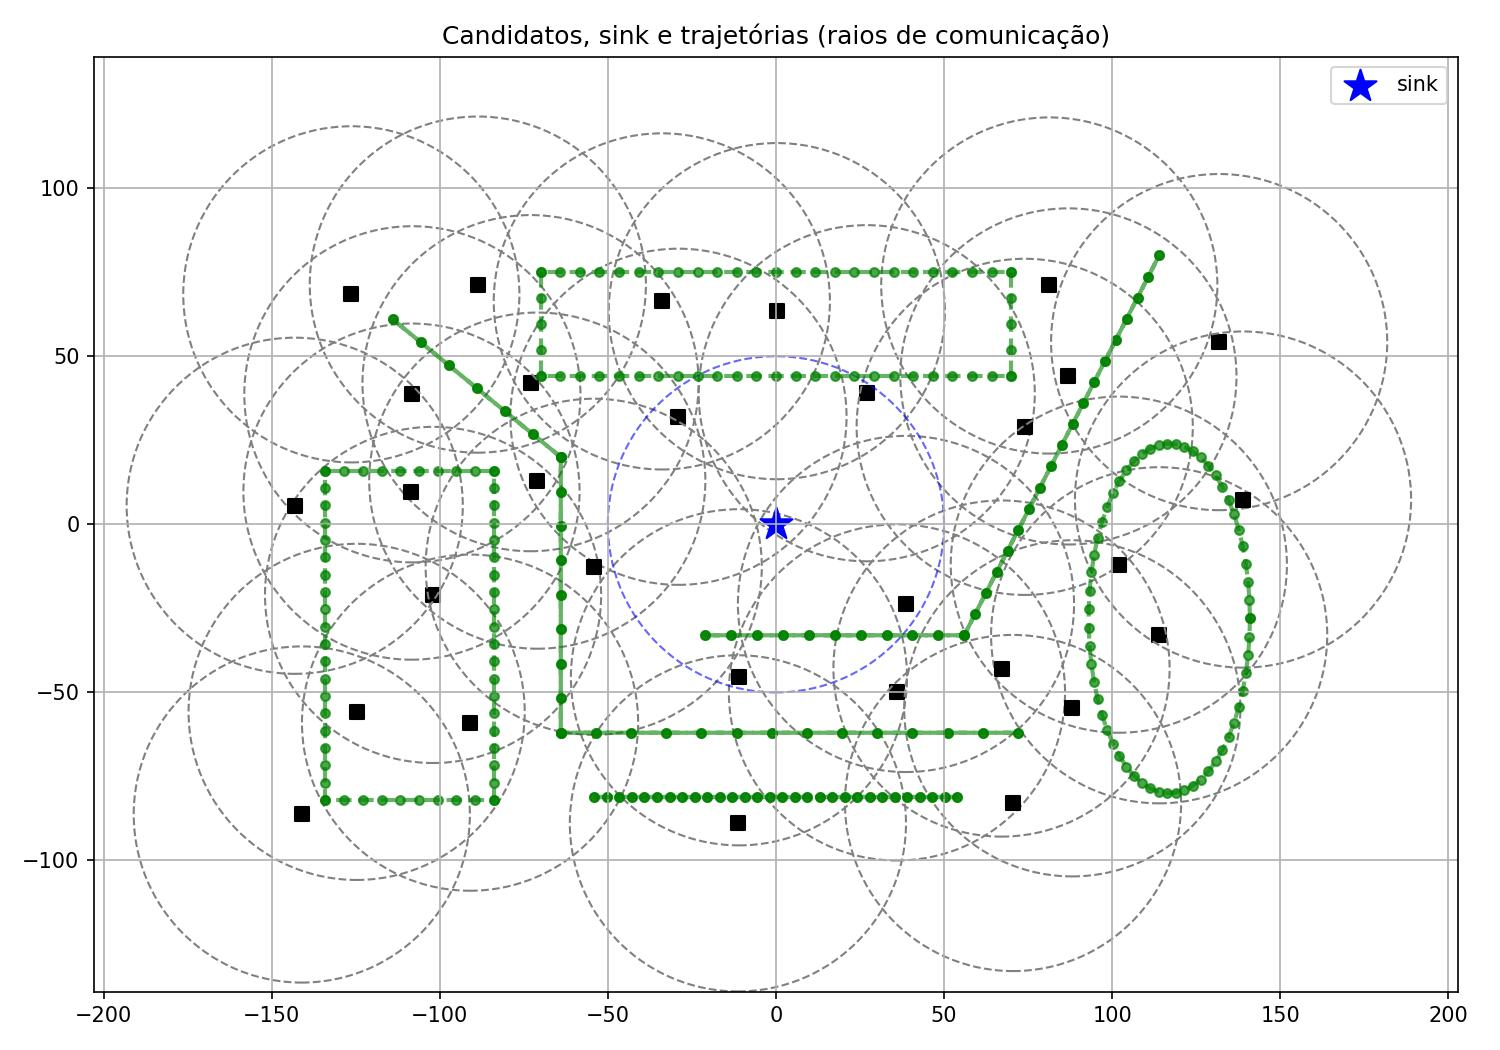
\includegraphics[height=4.7cm]{img/instancia.png}
  \end{figure}
  \note{Tempo: 45 segundos. Na Figura 2, mostre os candidatos como quadrados, o sink como estrela e as trajetórias em verde. Os círculos indicam alcance de comunicação. Os 90 metros de interferência se aplicam apenas à simulação. Esta é uma única instância controlada e os resultados devem ser interpretados nesse escopo.}
\end{frame}

\section{Resultados}

\begin{frame}{Resultados computacionais}
  \begin{center}
    \begin{tabular}{lr}
      \toprule
      \textbf{Indicador} & \textbf{Valor}\\
      \midrule
      Combinações na grade cartesiana & 2.750\\
      Execuções registradas & 1.626\\
      Execuções viáveis & 1.594\\
      Execuções inviáveis & 32\\
      Topologias distintas & 27\\
      Topologias com simulação compatível & 26\\
      \midrule
      Tempo médio de solução & 1,56 s\\
      Tempo máximo de solução & 4,60 s\\
      Gap máximo & 0,01\%\\
      \bottomrule
    \end{tabular}
  \end{center}
  \vfill
  As topologias geradas possuem entre 12 e 21 nós fixos instalados, com média de 16,6 nós.
  \note{Tempo: 65 segundos. Destaque que as 1594 execuções viáveis se reduzem a 27 instalações distintas. Das 27, 26 possuem correspondência exata com a campanha simulada; uma fica fora da análise operacional. Os tempos baixos se referem a esta instância e não demonstram escalabilidade. O gap máximo é 0,01 por cento; não afirme que todas as execuções tiveram prova exata de otimalidade. Fonte: Tabela 3 e Seção 4 do artigo.}
\end{frame}

\begin{frame}{Resultados da simulação}
  \begin{center}
    \small
    \begin{tabular}{lrrr}
      \toprule
      \textbf{Métrica} & \textbf{Mínimo} & \textbf{Média} & \textbf{Máximo}\\
      \midrule
      Latência (ms) & 65,44 & 126,37 & 188,51\\
      Energia (mJ) & 42.351 & 1.484.198 & 1.917.670\\
      Dados (bits) & 7.008 & 9.692 & 11.918\\
      \bottomrule
    \end{tabular}
  \end{center}
  \begin{figure}
    \centering
    % Painéis superiores da Figura 3. O arquivo mantém a figura completa.
    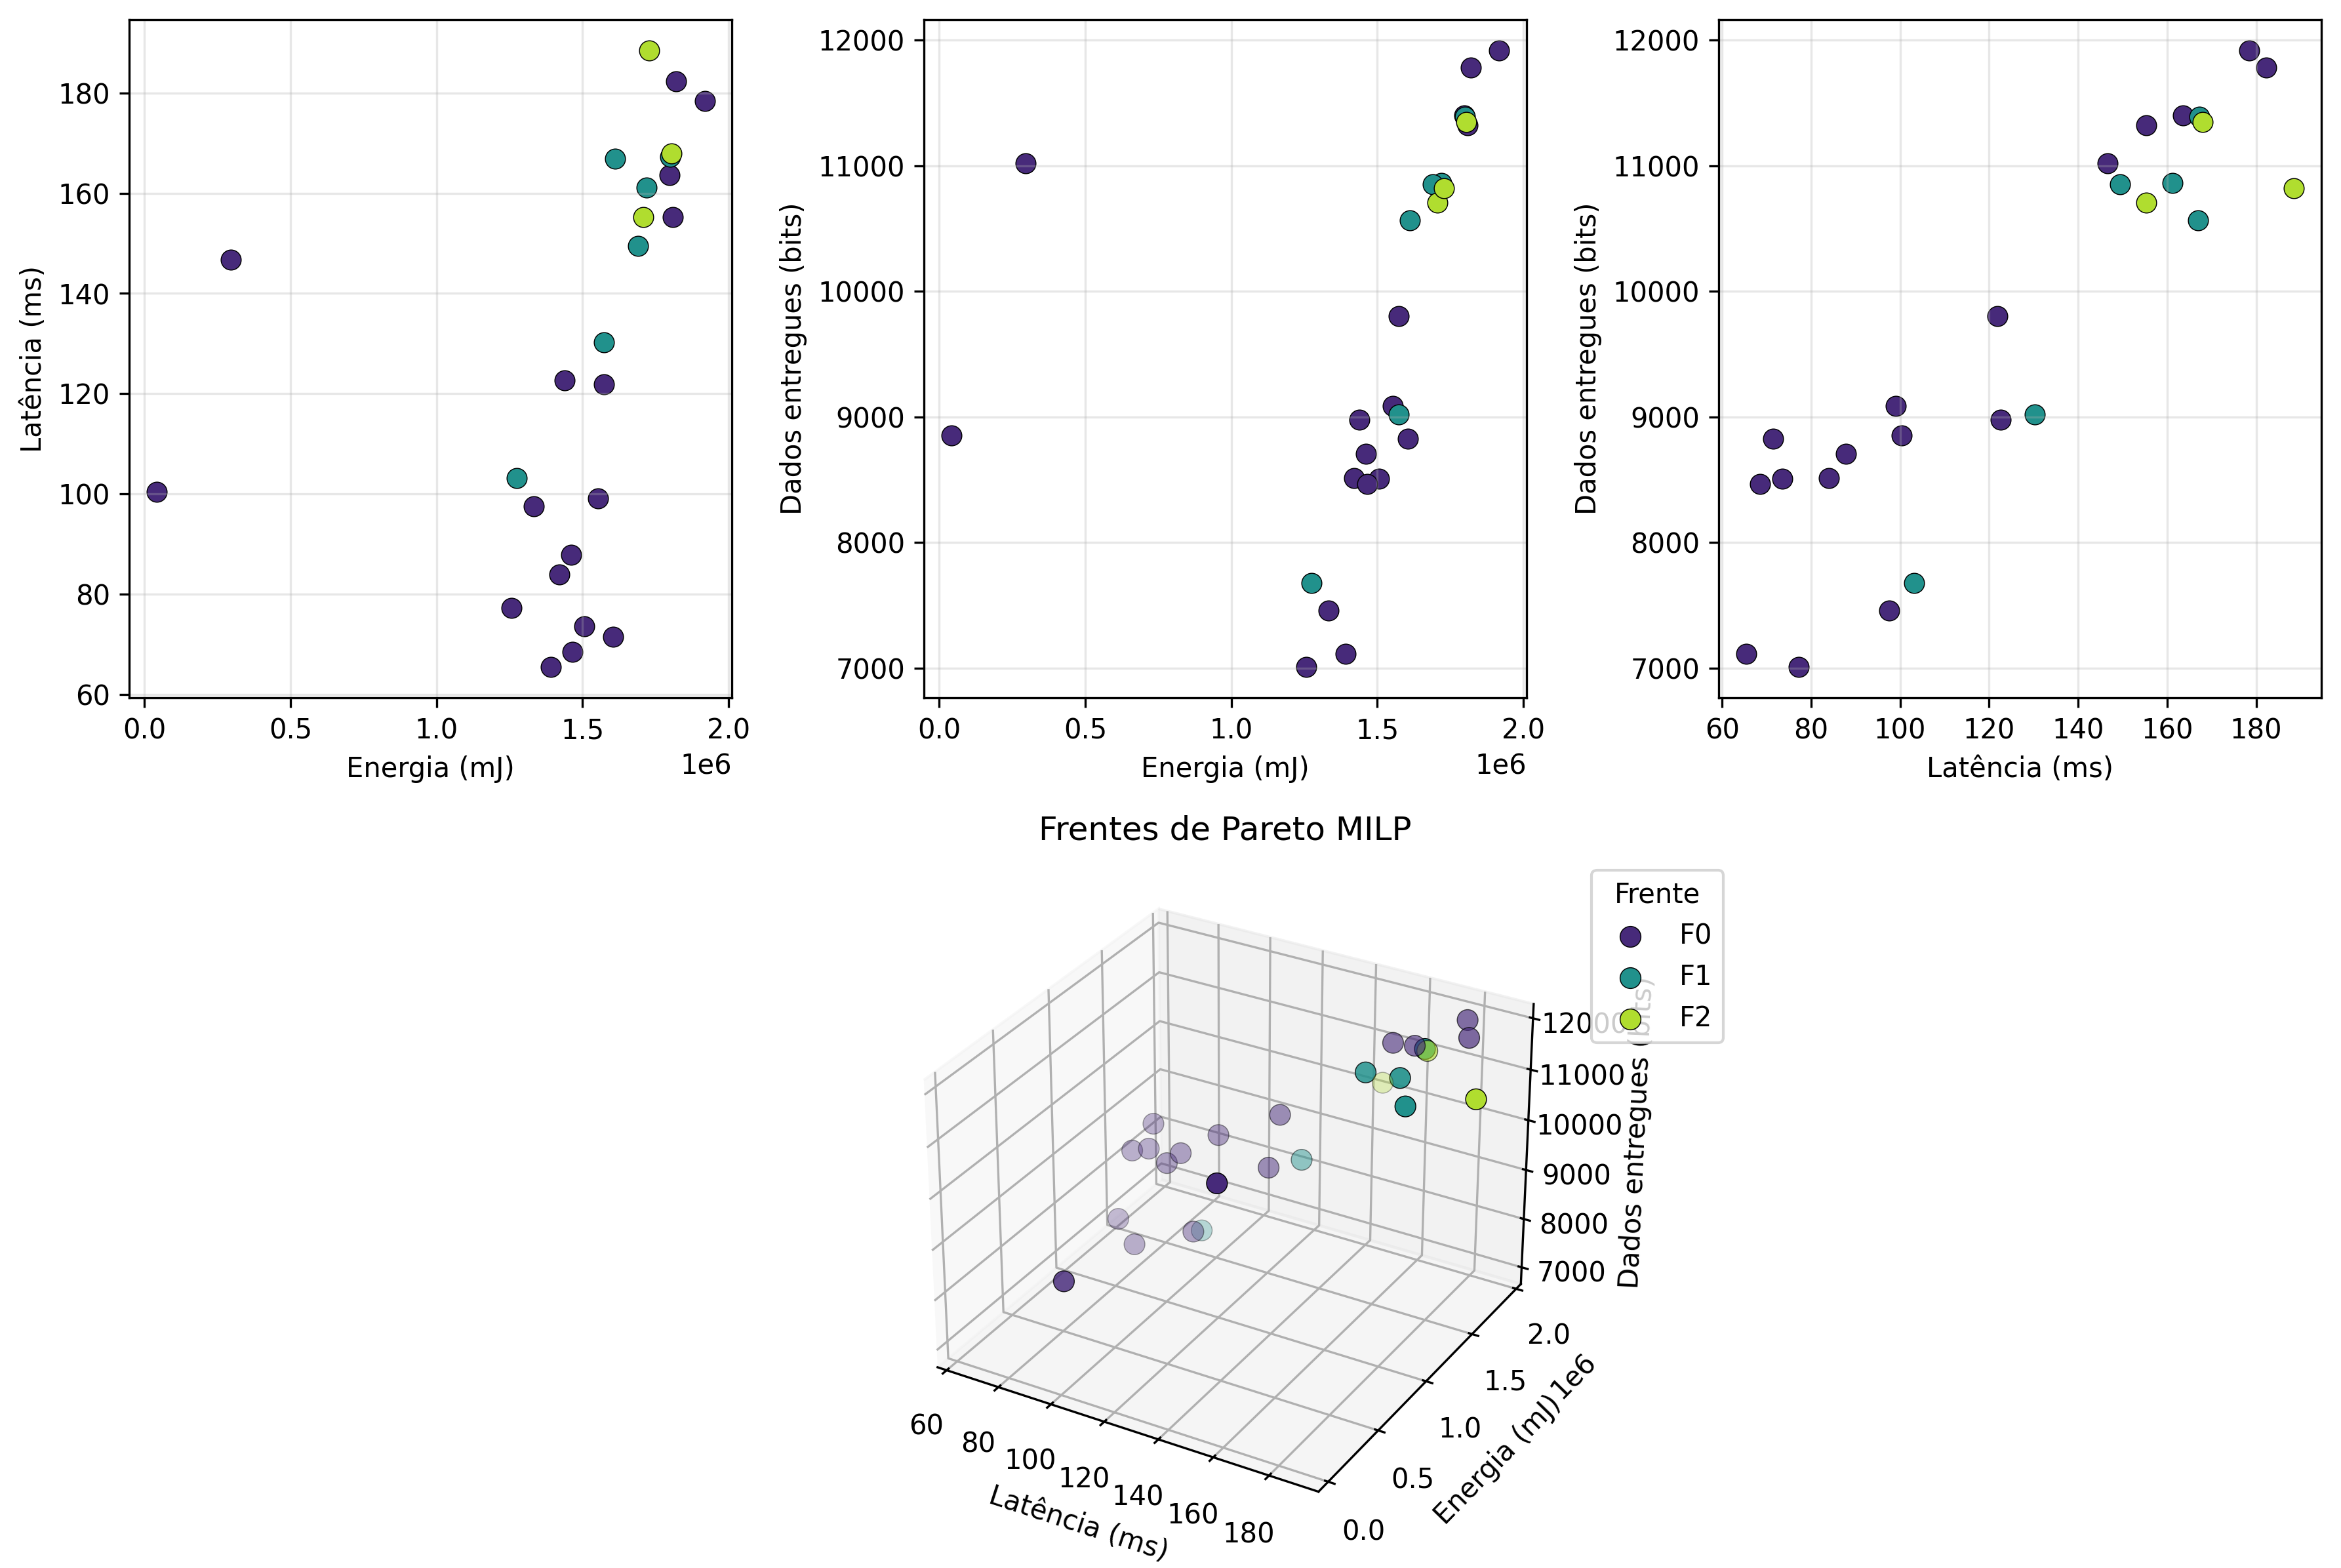
\includegraphics[width=.82\textwidth,trim=0 1170bp 0 0,clip]{img/frentes-pareto.png}
  \end{figure}
  \begin{itemize}
    \item Minimizar latência/energia e maximizar dados entregues.
    \item 17 topologias na primeira de três frentes de Pareto.
  \end{itemize}
  {\scriptsize Roxo: primeira frente; verde-azulado: segunda; verde-claro: terceira.}
  \note{Tempo: 75 segundos. Cada ponto é uma topologia. A classificação considera os três objetivos simultaneamente e foi feita após a simulação: o MILP possui objetivo escalar. Na primeira frente, nenhuma topologia é superada por outra em todos os critérios no sentido de dominância. Não há uma única rede que domine todas as demais. Os extremos da tabela podem pertencer a redes diferentes. As cores se referem à análise em três dimensões, mesmo nas projeções bidimensionais. Fonte: Tabela 4 e Figura 3 do artigo.}
\end{frame}

\begin{frame}{Estrutura das topologias e desempenho}
  \begin{figure}
    \centering
    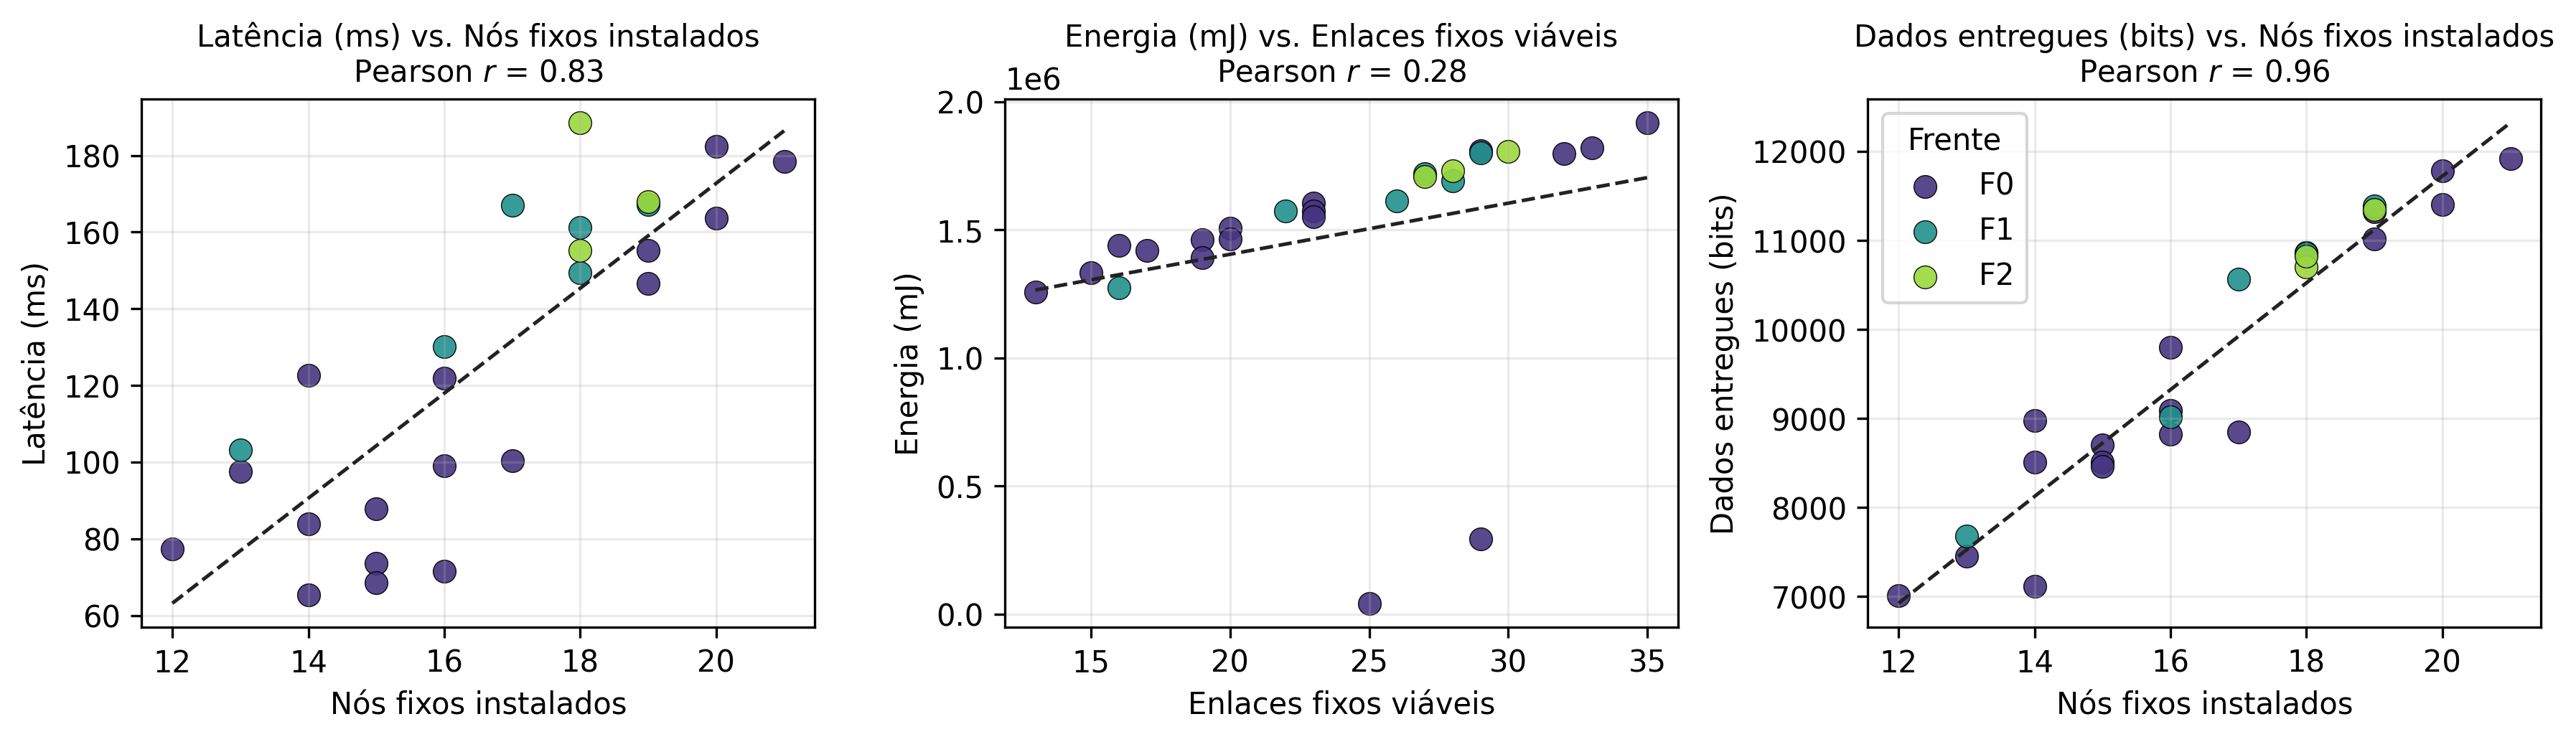
\includegraphics[width=\textwidth]{img/correlacoes.png}
  \end{figure}
  \begin{itemize}
    \item Número de nós instalados: correlação com latência ($r=0{,}83$) e dados entregues ($r=0{,}96$).
    \medskip
    \item Enlaces fixos viáveis: associação mais fraca com energia ($r=0{,}28$).
  \end{itemize}
  \begin{block}{Variação da demanda no MILP}
    Entre as faixas baixa e alta de $B$, os dados médios entregues passaram de 9.250 para 10.328 bits, e a latência média de 114,65 para 140,97 ms.
  \end{block}
  \note{Tempo: 70 segundos. A Figura 4 mostra associações entre estrutura e desempenho nas 26 topologias. Mais nós se associam a mais dados e maior latência; a relação com energia é menos explicada pelo descritor selecionado. Correlação não demonstra causalidade. Entre baixa e alta demanda B, a média de nós passa de 15,8 para 17,9. B é parâmetro do MILP, não uma taxa de tráfego equivalente no simulador. Esses resultados são tendências preliminares.}
\end{frame}

\section{Considerações finais}

\begin{frame}{Considerações finais}
  \begin{itemize}
    \item O MILP integra instalação de nós fixos, habilitação de enlaces e roteamento ao longo de trajetórias discretizadas.
    \medskip
    \item A viabilidade estrutural não determina, isoladamente, latência, energia e entrega de dados na simulação.
    \medskip
    \item A avaliação é preliminar: uma instância e 26 topologias simuladas, sem comparação operacional com os baselines.
  \end{itemize}
  \begin{block}{Trabalhos futuros}
    Ampliar as instâncias consideradas, estender o modelo e explorar a otimização multiobjetivo, utilizando-o também como mecanismo de verificação de viabilidade integrado ao NSGA.
  \end{block}
  \note{Tempo: 80 segundos. Retome a contribuição: o modelo gera instalações viáveis e a simulação avalia seus compromissos operacionais. Alguns detalhes da campanha de simulação não estão disponíveis para documentação completa. All-Candidates ativa todos os candidatos, e Random-k escolhe k posições aleatórias; sem métricas simuladas correspondentes, não se pode afirmar superioridade sobre essas referências. Conclua com os próximos passos, sem voltar às equações.}
\end{frame}

\begin{frame}[plain]
  \vfill
  \begin{beamercolorbox}[sep=8pt,center,shadow=true,rounded=true]{title}
    \usebeamerfont{title}Obrigado!\par
  \end{beamercolorbox}
  \medskip
  \begin{center}
    Junio Cesar Ferreira\\
    \href{mailto:juniocesarferreira@usp.br}{juniocesarferreira@usp.br}
  \end{center}
  \vfill
  {\footnotesize
    \textbf{Agradecimentos}\\
    FAPESP: processos 2020/09770-7 e 2021/06968-3.\\
    CNPq: processo 444791/2024-8 -- Conhecimento Brasil.
  }
  \note{Tempo: 20 segundos. Agradeça a atenção, os coautores e as agências de fomento. Abra para perguntas. O roteiro completo, incluindo as seis aberturas de seção, totaliza 15 minutos, sem contar a discussão.}
\end{frame}

\end{document}
